\documentclass[14pt,xcolor=dvipsnames,table,dvipdfmx]{beamer}

\setbeamertemplate{bibliography item}[text]
\usepackage[absolute,overlay]{textpos}
\usepackage{apalike}
\usetheme{Boadilla}

\usepackage{txfonts} % TXフォント
\renewcommand{\kanjifamilydefault}{\gtdefault}  % 日本語をゴシック体に
\usefonttheme{structurebold} % タイトル部を太字
\setbeamerfont{alerted text}{series=\bfseries} % Alertを太字
\setbeamerfont{section in toc}{series=\mdseries} % 目次は太字にしない
\setbeamerfont{frametitle}{size=\Large} % フレームタイトル文字サイズ
\setbeamerfont{title}{size=\LARGE} % タイトル文字サイズ
\setbeamerfont{date}{size=\small}  % 日付文字サイズ
\usepackage{pxjahyper}

\uselanguage{japanese}
\languagepath{japanese}
\deftranslation[to=japanese]{Theorem}{定理}
\deftranslation[to=japanese]{Lemma}{補題}
\deftranslation[to=japanese]{Example}{例}
\deftranslation[to=japanese]{Examples}{例}
\deftranslation[to=japanese]{Definition}{定義}
\deftranslation[to=japanese]{Definitions}{定義}
\deftranslation[to=japanese]{Problem}{問題}
\deftranslation[to=japanese]{Solution}{解}
\deftranslation[to=japanese]{Fact}{事実}
\deftranslation[to=japanese]{Proof}{証明}
\def\proofname{証明}

\definecolor{UniBlue}{RGB}{0,150,200} 
\definecolor{AlertOrange}{RGB}{255,76,0}
\definecolor{AlmostBlack}{RGB}{38,38,38}
\setbeamercolor{normal text}{fg=AlmostBlack}  % 本文カラー
\setbeamercolor{structure}{fg=UniBlue} % 見出しカラー
\setbeamercolor{block title}{fg=UniBlue!50!black} % ブロック部分タイトルカラー
\setbeamercolor{alerted text}{fg=AlertOrange} % \alert 文字カラー
\mode<beamer>{
    \definecolor{BackGroundGray}{RGB}{254,254,254}
    \setbeamercolor{background canvas}{bg=BackGroundGray} % スライドモードのみ背景をわずかにグレーにする
}

% Algorithm系
\usepackage{algorithm}
\usepackage[noend]{algorithmic}
\algsetup{linenosize=\color{fg!50}\footnotesize}
\renewcommand\algorithmicdo{:}
\renewcommand\algorithmicthen{:}
\renewcommand\algorithmicrequire{\textbf{Input:}}
\renewcommand\algorithmicensure{\textbf{Output:}}
\newcommand{\argmin}{\operatornamewithlimits{argmin}}
\newcommand{\argmax}{\operatornamewithlimits{argmax}}
%フラットデザイン化
\setbeamertemplate{blocks}[rounded] % Blockの影を消す
\useinnertheme{circles} % 箇条書きをシンプルに
\setbeamertemplate{navigation symbols}{} % ナビゲーションシンボルを消す
\setbeamertemplate{footline}[frame number] % フッターはスライド番号のみ

\AtBeginSection[]{
    \frame{\tableofcontents[currentsection, hideallsubsections]} %目次スライド
}

\newcommand{\tabincell}[2]{\begin{tabular}{@{}#1@{}}#2\end{tabular}}

\title{\bfseries 特許検索における質問意図の曖昧化}

\date{2016年1月31日}
\author{中川研 胡 瀚林 \\ 指導教員:中川 裕志 教授}
%\subject{PIR}
%\keywords{PIR,Obfuscation,query}

\begin{document}

\maketitle
\frame{\tableofcontents[hideallsubsections]}


\section{背景紹介}
\begin{frame}{特許}
	\begin{block}{特許とは?}
		\begin{itemize}
        \item 特許法第1条には,「この法律は、発明の保護及び利用を図ることにより,発明を奨励し,もつて産業の発達に寄与することを目的とする」とある.
		\item 特許制度は,発明者には一定期間,一定の条件のもとに特許権という独占的な権利を与えて発明の保護を図る一方,その発明を公開して利用を図ることにより新しい技術を人類共通の財産としていくことを定めて,これにより技術の進歩を促進し,産業の発達に寄与しようというものである.
		\end{itemize}
	\end{block}
\end{frame}

\begin{frame}{特許}
	\begin{block}{特許を取る条件}
		\begin{itemize}
			\item {\em (新規性:特許法29条第1項)}特許出願前に公然知られた発明,
			公然実施をせれた発明,頒布された刊行物に記載された発明又は
			電気通信回線を通じて公衆に利用可能となった発明について特許を受けることができない.
 			\item {\em (進歩性:特許法29条第2項)}特許出願前にその発明の属する技術の分野における通常の知識を有する者
			が前項各号に掲げる発明に基いて容易に発明をすることができたときは,その発明については、同項の規定にかかわらず,特許を受けることができない.
		\end{itemize}
	\end{block}
\end{frame}


\end{document}

\begin{frame}{特許}
    \begin{exampleblock}{特許請求の範囲}
		【請求項1】植物の種子をパルプ繊維の水懸濁液に混合して抄紙する播種シートの製造方法。\\
		【請求項2】水懸濁液にさらに水溶性接着剤を添加する請求項1記載の播種シートの製造方法。\\
		【請求項3】あらかじめ種子を低粘度多価アルコールで被覆する請求項1記載の播種シートの製造方法。
    \end{exampleblock}
	\begin{block}{特許請求の範囲の作成方法}
		8技術用語は、学術用語を用いる。\\
		9用語は、その有する普通の意味で使用し、かつ、明細書及び特許請求の範囲全体を通じて統一して使用する	
	\end{block}
\end{frame}

\begin{frame}{国際特許分類}
	\begin{exampleblock}{\center A61C 5/08A}
	\begin{tabular}{cc}
	セクション:A & 健康および娯楽 \\
 	サブセクション : 61 & 医学または獣医学:衛生学 \\
 	クラス: C & 歯科:口腔または歯科衛生 \\
 	メイングループ:5 & 歯の充填または被覆 \\
 	サブグループ:08 & 歯冠:その製造;口中での歯冠固定 \\
	\end{tabular}
	\end{exampleblock}
	\begin{block}{}
		全ての特許が人の手によって分類されている
	\end{block}
\end{frame}

\begin{frame}{特許検索}
	\begin{block}{}
		\fontsize{8pt}{7.2}\selectfont
		\begin{tabular}{ccc}
        \noalign{\hrule height 1pt}
        検索タイプー & 検索対象(specification) & 検索目的 \\
        \hline
        \tabincell{c}{技術水準調査\\(State of the Art Search)} & イデア & 自分の発明に関連する背景知識を得る \\
        \tabincell{c}{新規性調査\\(Novelty Search)} & 特許文章 & 特許登録の可能性を判断する \\
        \tabincell{c}{侵害調査\\(Infringement Search)} &  \tabincell{c}{商品と\\商品に関連する技術} & 権利侵害とならないかを判断する \\
        \noalign{\hrule height 1pt}
        \end{tabular}
	\end{block}
\end{frame}

\begin{frame}{新規性調査}
\begin{columns}[t]
    \begin{column}{0.8\textwidth} % 横幅の30%
      	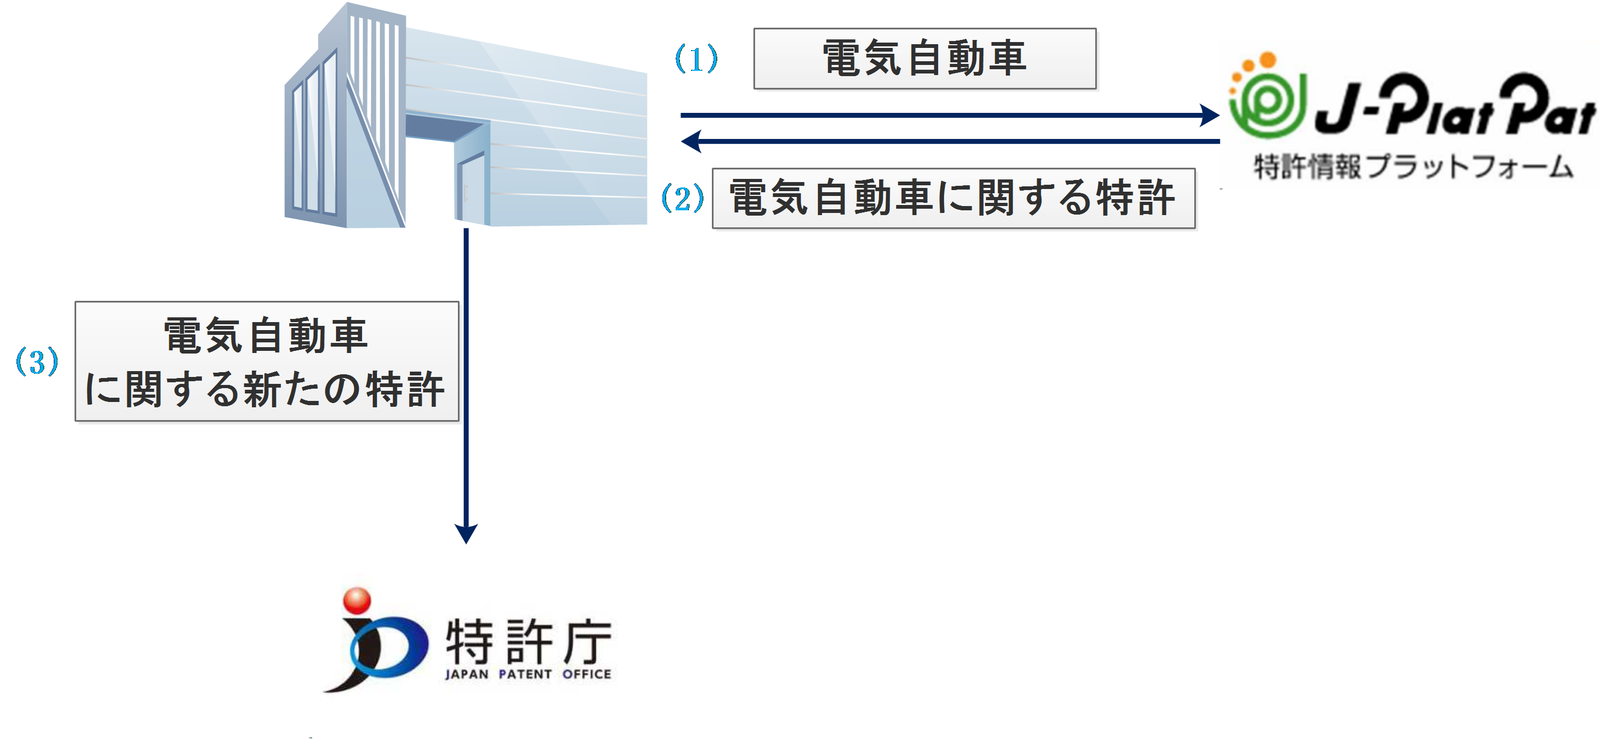
\includegraphics[width=\columnwidth]{rk1.png}
    \end{column}
\end{columns}
\end{frame}

\begin{frame}{新規性調査}
\begin{columns}[t]
    \begin{column}{0.8\textwidth} % 横幅の30%
      	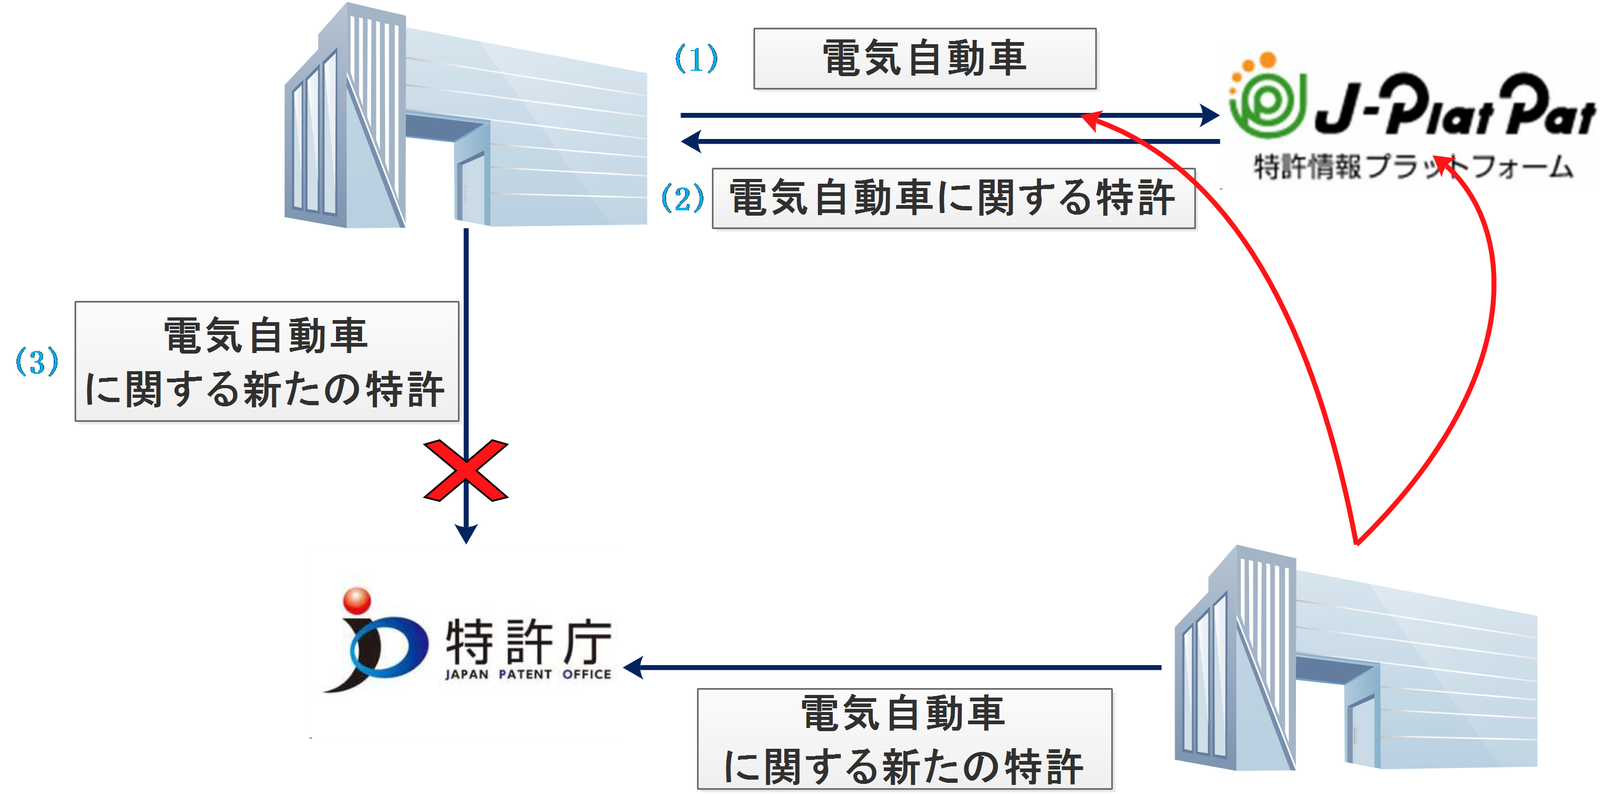
\includegraphics[width=\columnwidth]{rk2.png}
    \end{column}
\end{columns}
\end{frame}

\begin{frame}{特許検索質問}
	\fontsize{10pt}{7.2}\selectfont
	\begin{exampleblock}{播種シートの製造方法}
		植物 種子 パルプ 繊維 水 液 混合 抄 紙 播種 シート 製造 方法 水溶 性 接着 剤 添加 記載 度 価 アルコール 被覆
	\end{exampleblock}
	\fontsize{14pt}{7.2}\selectfont
	\begin{block}{}
    \begin{itemize}
		\item 請求項から名詞を取り出し,検索質問とする
        \item 検索質問は単語(名詞)の集合である
        \item 質問に含む単語数が多い
		\begin{itemize}
			\item ウェブ検索:2.35 特許検索:20.1
		\end{itemize}
		\item 専門用語が多い
    \end{itemize}
	\end{block}
\end{frame}

\begin{frame}{テキスト検索}
\begin{columns}[t]
    \begin{column}{0.8\textwidth} % 横幅の30%
        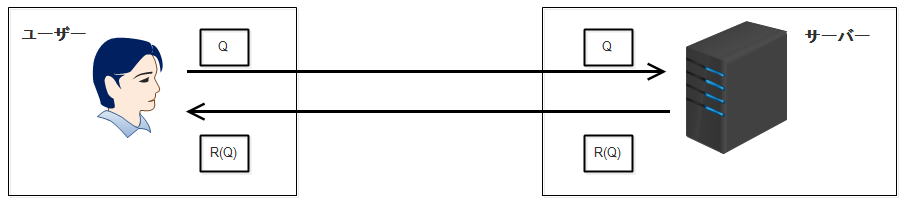
\includegraphics[width=\columnwidth]{photo1.png}
    \end{column}
\end{columns}
    \begin{block}{}
    \begin{itemize}
        \item 検索質問$q$:単語の集合
        \item 質問$q$の検索結果$R(Q)$:文章の集合
    \end{itemize}
    \end{block}
\end{frame}

\begin{frame}{Obfuscation Search}
    \begin{columns}[t]
        \begin{column}{1\textwidth} % 横幅の30%
            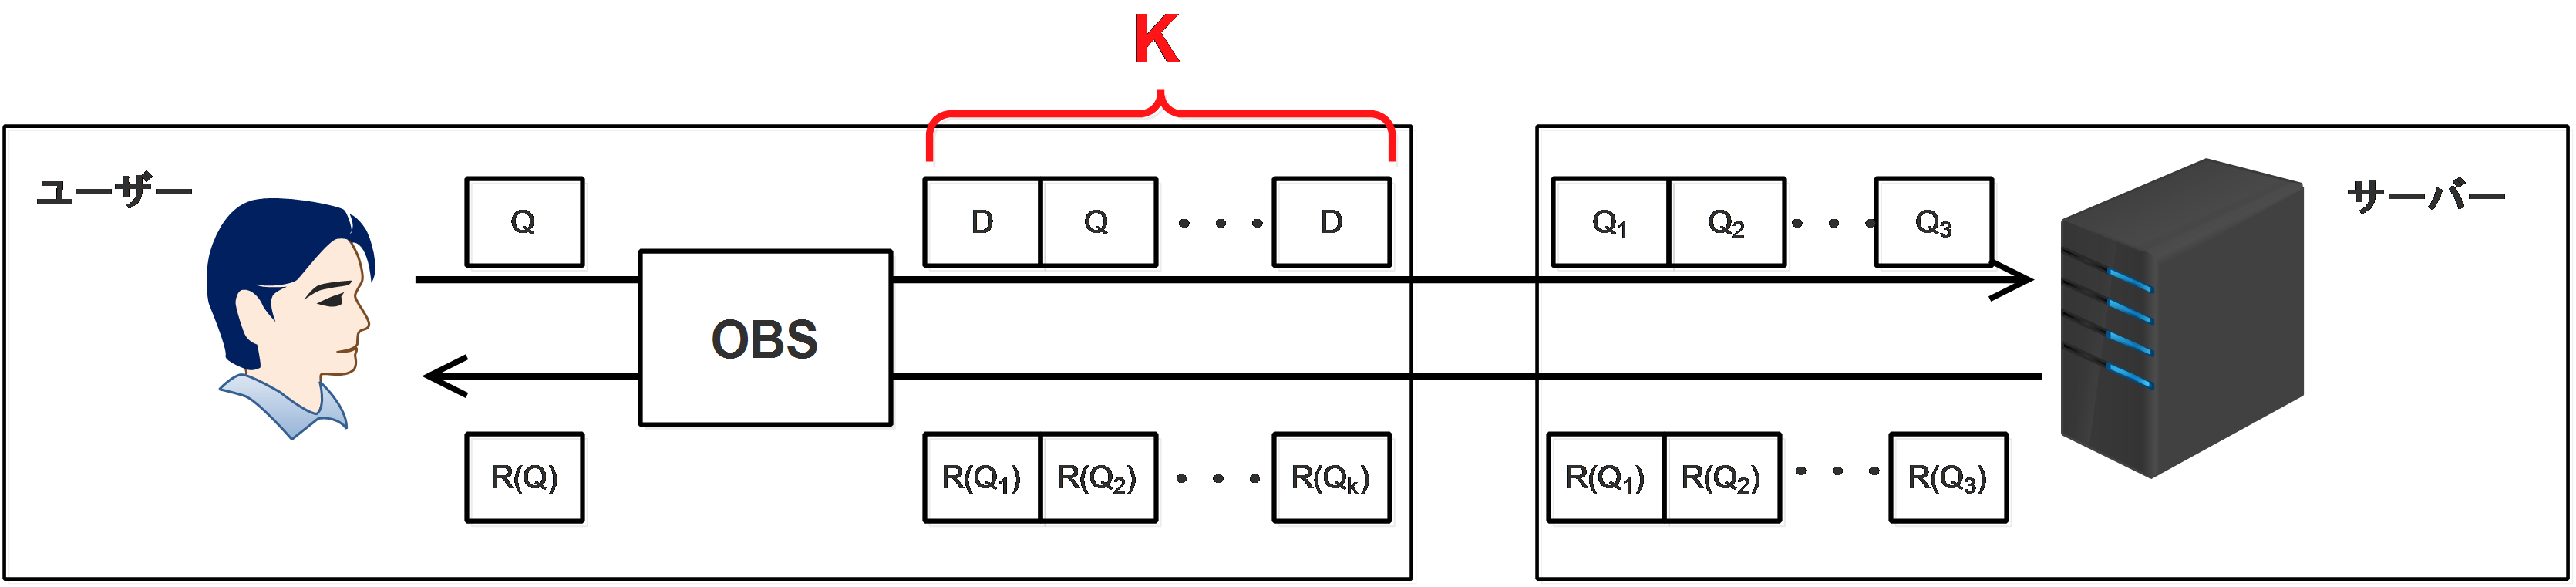
\includegraphics[width=\columnwidth]{rk4.png}
		\end{column}
    \end{columns}
	\begin{block}{} 
		\begin{itemize}
			\item 真の質問と$K-1$個真の質問と区別できないダミー質問と同時に検索する
			\item サーバーが真の質問を見つける確率が$1/k$
		\end{itemize}
	\end{block}
\end{frame}

\begin{frame}{Obfuscation Search:例}
    \begin{columns}[t]
        \begin{column}{1\textwidth} % 横幅の30%
            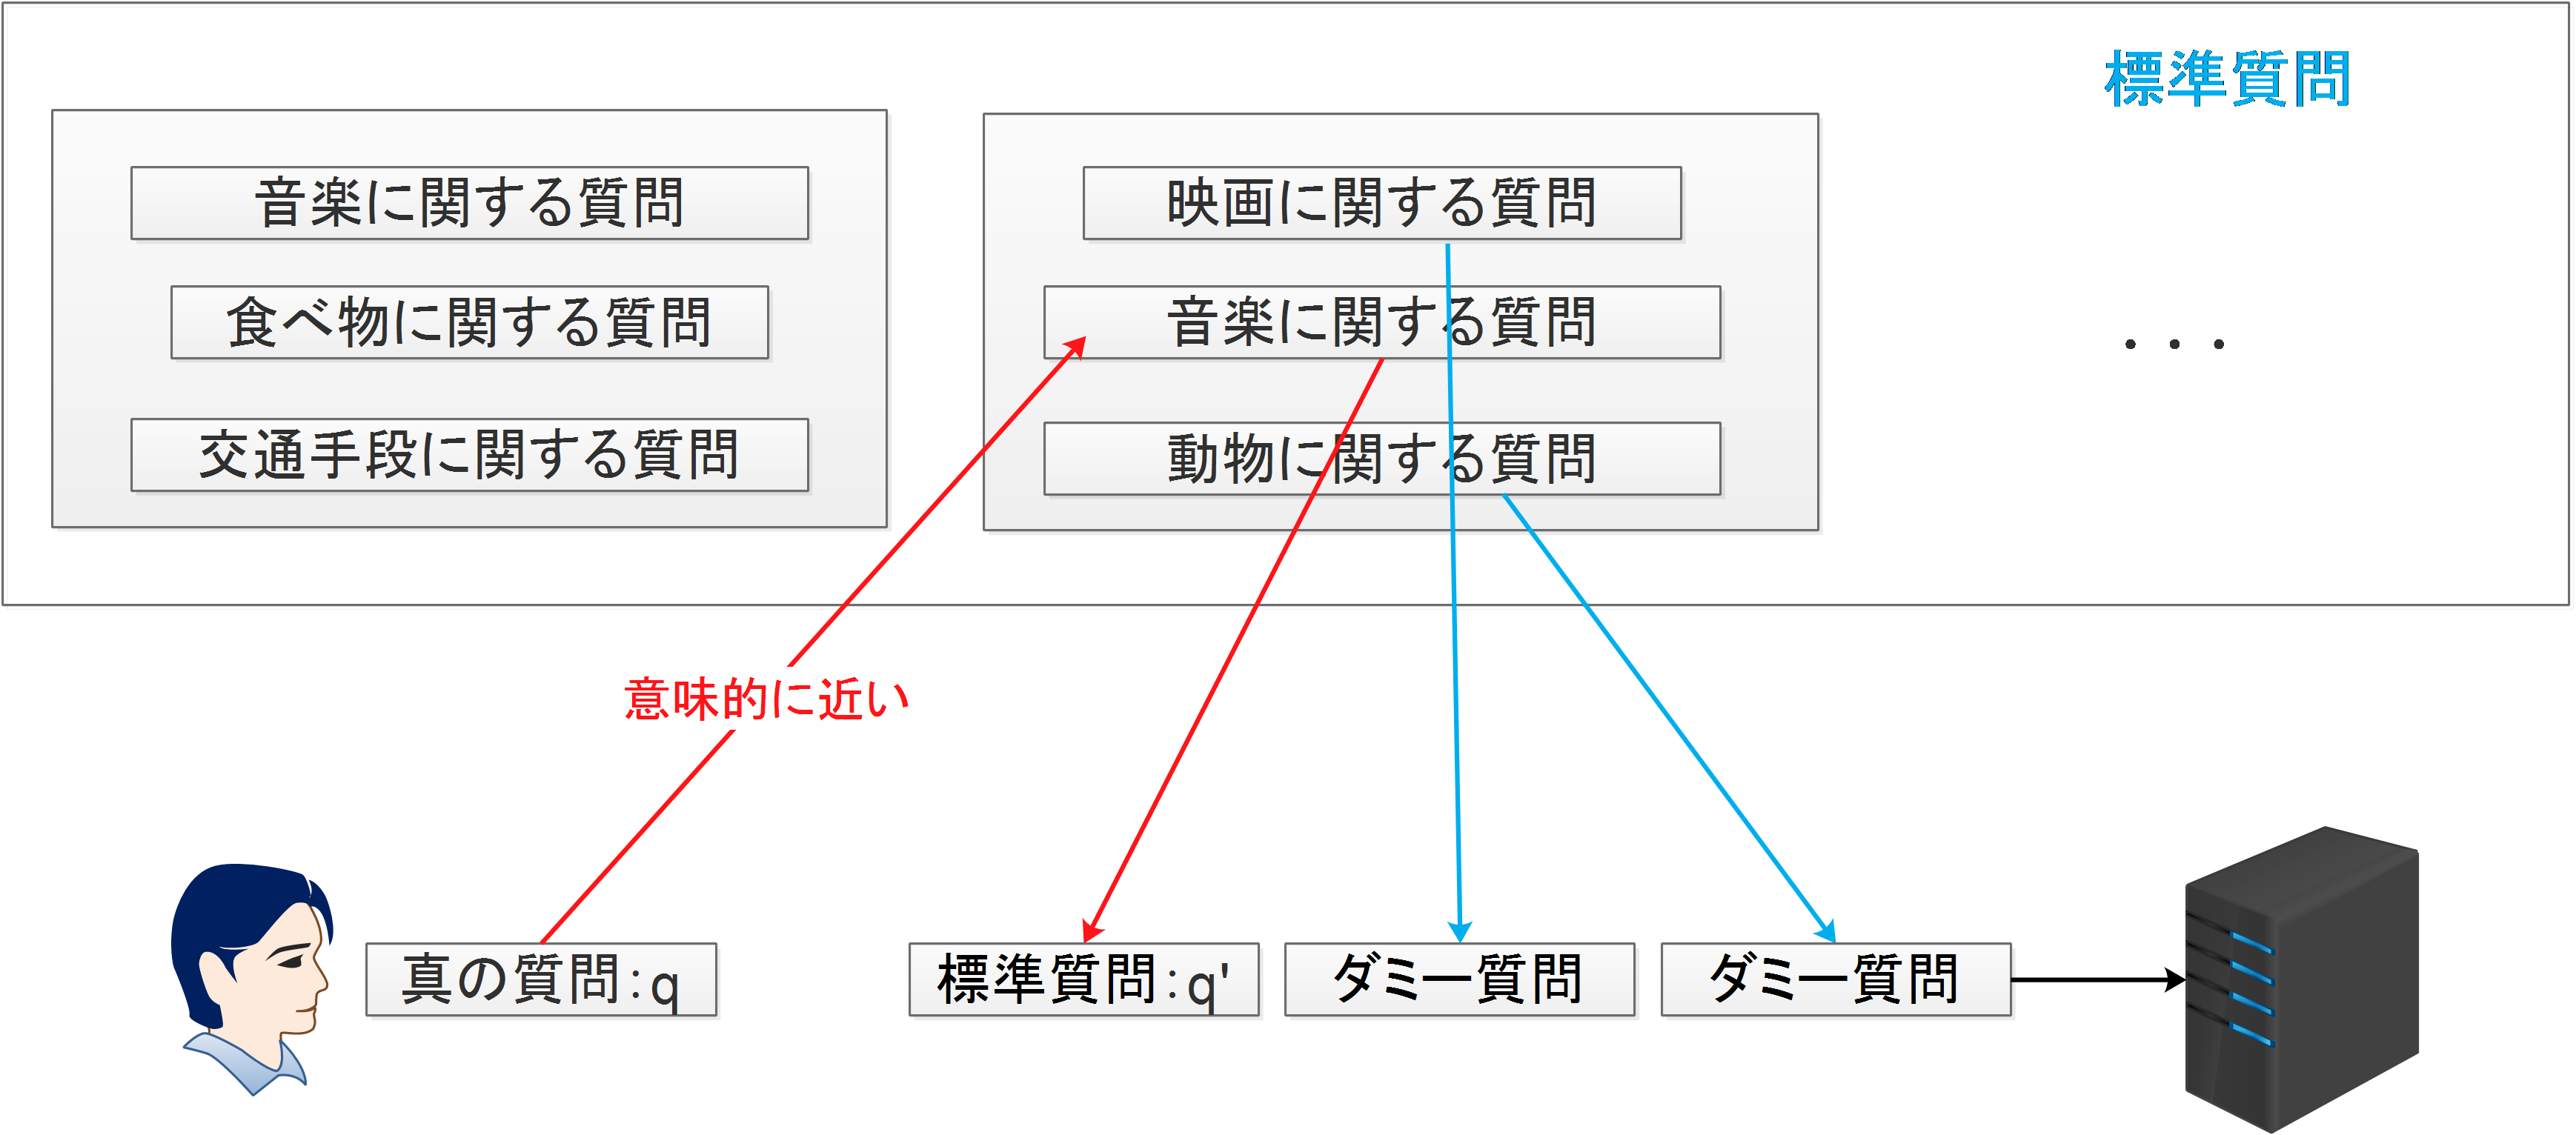
\includegraphics[width=\columnwidth]{rk14.png}
		\end{column}
    \end{columns}
	\begin{block}{} 
		\begin{itemize}
			\item 実践的には長い質問に対応できない
			\item 質問$q'$を使うことより検索の精度と再現率が下がる
		\end{itemize}
	\end{block}
\end{frame}

\begin{frame}{Obfuscation Search}
\fontsize{12pt}{7.2}\selectfont
    \begin{block}{ユニバーサル質問集合:$Q$}
		$W$を全ての単語の集合とする.
		ユニバーサル質問集合$Q$とは$W$の冪集合である,つまり
		\begin{equation}
		Q = P(W) = \{X|X \subset W\}
		\end{equation}
    \end{block}
    \begin{block}{質問-トピックスコア関数:$rscore$}
		$T$を全ての可能なトピックの集合とする.
		質問$q$とトピック$t$の関係を表す関数とは
		\begin{equation}
		rscore:Q \times T \to \mathbb{R}
		\end{equation}
    \end{block}
    \begin{block}{質問間距離関数:$dist$}
		質問$q_1$と質問$q_2$間の距離を表す関数とは
		\begin{equation}
		dist:Q \times Q \to \mathbb{R}
		\end{equation}
    \end{block}
\end{frame}

\begin{frame}{目標}
    \begin{block}{}
    \begin{itemize}
        \item 長い質問に対応できる
        \item 専門用語が多いダミーを生成できる
		\item 検索の精度と再現率を維持できる
    \end{itemize}
    \end{block}
\end{frame}

\section{既存研究}
\begin{frame}{Providing Privacy through Plausibly Deniable Search \cite{providing2009}}
	\begin{block}{}
	質問$q$をユーザーが入力した質問とする.ダミー質問生成システム$D$が$k$個の質問を含んでいる質問集合$D(q_u)=\{q_1, \dots , q_k\}$を出力しサー
	バーに提出する.$D(q_u)$が以下の性質を持つなら,$D(q_u)$をPD-質問集合といい,$D$を$k$−否認可能検索という
	\begin{enumerate}
	\item $\exists q_i \in D(q_u),q_i$と$q_u$が意味的に近い
	\item $\forall q_j \in D(q_u),D(q_j) = D(q_u)$
	\item $\forall q_j \in D(q_u),q_j$が違うトピックに含まれる
	\item $\forall q_j \in D(q_u),q_j$が同じような尤もらしさを持つ
	\end{enumerate}
	\end{block}
\end{frame}

\begin{frame}{Latent Semantic Indexing}
    \begin{columns}[c]
        \begin{column}{1.0\textwidth} % 横幅の30%
            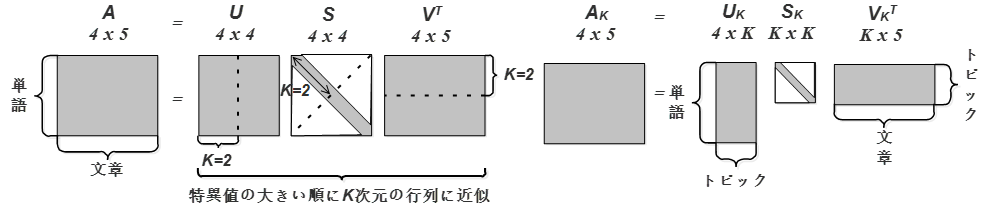
\includegraphics[width=\columnwidth]{photo11.png}
		\end{column}
    \end{columns}
	\begin{block}{潜在的意味インデキシング}
	\fontsize{12pt}{7.2}\selectfont
		単語$\cdot$文書行列$A$の$(i,j)$番目の要素は$i$番目の単語が$j$番目の文章に出現した回数である \\
		$A$を特異値分解$A = USV^T$し、$U$、$S$、$V$	の各列ベクトルを特異値が大きい順に
		$K$個用いて$A$の低ランク近似$A_K=U_KS_KV_{K}^T$を得る \\
		このように低ランク分解によって、単語とトピックの関係を分析できる \\
		$A_K$の$(i,j)$番目の要素は$i$番目の単語と$j$番目のトピックの関係を表す
	\end{block}
\end{frame}

\begin{frame}{Providing Privacy through Plausibly Deniable Search \cite{providing2009}}
	\fontsize{12pt}{7.2}\selectfont
	\begin{block}{質問-トピックスコア関数:$rscore_{LSI}$}
		$S_K$を単語$\cdot$文書行列$A$の低ランク近似の結果とし,
		$S_K(i,j)$を$S_K$の$(i,j)$番目の要素とする.
		$LSI$による質問$q$とトピック$t$の関係を表す関数とは
		\begin{equation}
			rscore_{LSI}(q,t) = \sum_{w \in q}S_K(w,t)
		\end{equation}
	\end{block}
	\begin{block}{質問間距離関数:$dist_{LSI}$}
		$LSI$による質問$q_1$と質問$q_2$の距離を表す関数とは
		\begin{equation}
			dist_{LSI}(q_1,q_2) = 1-\frac{\sum_{t \in T}rscore_{LSI}(q_1,t) \cdot rscore_{LSI}(q_2,t)}{\sum_{t \in T}(rscore_{LSI}(q_1,t^2))^{1/2}+\sum_{t \in T}(rscore_{LSI}(q_2,t)^2)^{1/2}}
		\end{equation}
	\end{block}
\end{frame}

\begin{frame}{Providing Privacy through Plausibly Deniable Search \cite{providing2009}}
	\begin{columns}[t]
		\begin{column}{0.95\textwidth} % 横幅の30%
			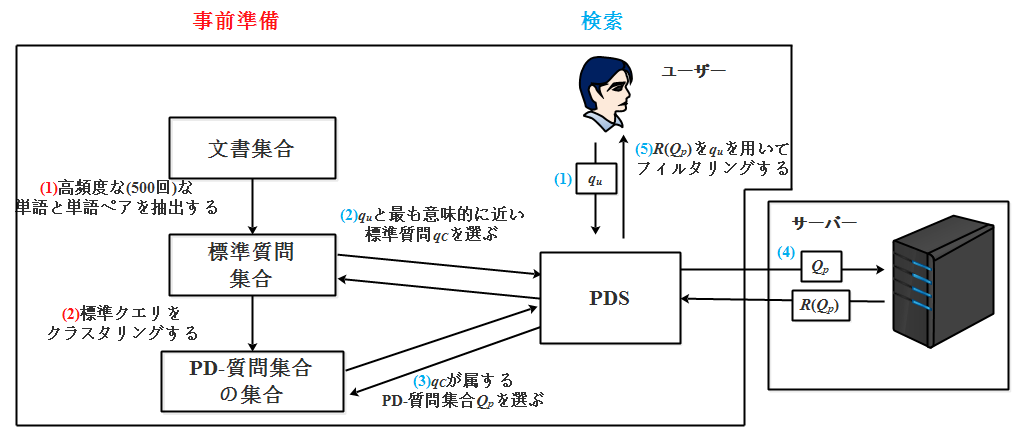
\includegraphics[width=\columnwidth]{th01.png}
		\end{column}
	\end{columns}
\end{frame}

\begin{frame}{Providing Privacy through Plausibly Deniable Search \cite{providing2009}}
	\begin{block}{問題点}
		\begin{itemize}
			\item 	質問の長さの増加に伴って標準質問の数が指数的に増加するため,長い質問対応できない
			\item 	真の質問ではなく,真の質問に意味的に近い標準質問を用いるため,精度と再現率が低い
			\item 	\cite{providing2009}ではPD-質問集合を作るときは質問間で距離しか配慮していないため、
					同じトピックについて複数検索すると真の質問が属するトピック出現回数がほかのトピックより多くなる.
					したがって出現回数が一番多いトピックに属する質問が真の質問となる可能性が大きい.
		\end{itemize}
	\end{block}
\end{frame}

\begin{frame}{Embellishing Text Search Queries to Protect User Privacy \cite{embellishing2010}}
	\begin{block}{}
		\begin{itemize}
			\item	質問の全体ではなく単語ごとにダミー単語を混ぜる.
			\item	単語バケットを事前に作り,真の質問の単語と同じバケットにある他の単語をダミー単語とする.
		\end{itemize}
	\end{block}
	\begin{block}{バケット作り}
		\begin{itemize}
			\item	同じバケットにある単語の特殊さは近いが,意味的には大きい違いがある. 
			\item	任意の2つのバケットの全ての単語間の意味的距離の差が近い
		\end{itemize}
	\end{block}
\end{frame}

\begin{frame}{Wordnet}
\fontsize{12pt}{7.2}\selectfont
	\begin{columns}[t]
		\begin{column}{1.0\textwidth} % 横幅の30%
			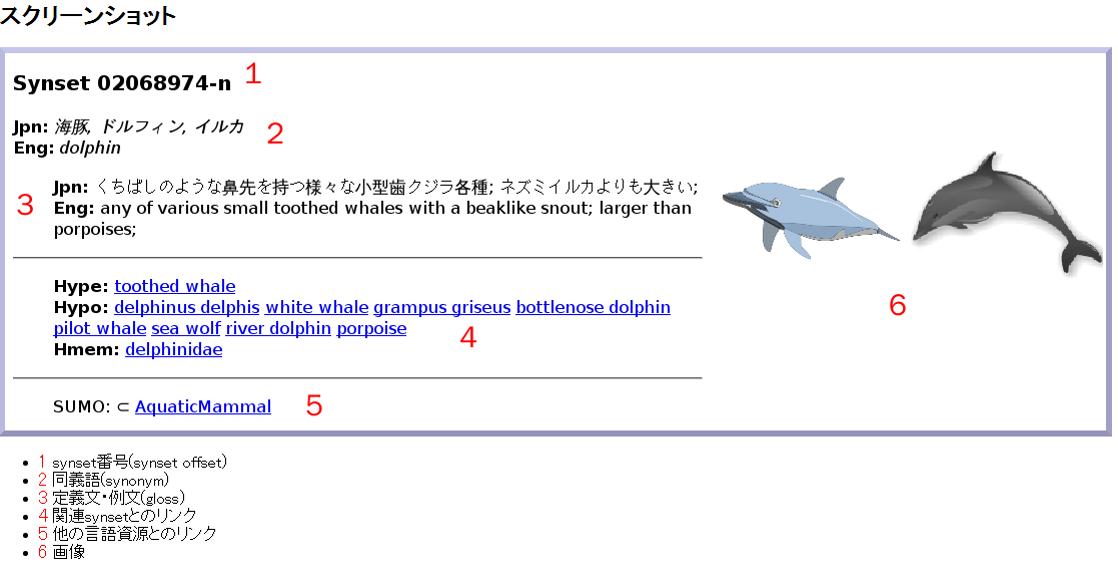
\includegraphics[width=\columnwidth]{photo14.png}
		\end{column}
	\end{columns}
	\begin{block}{}
		単語を類義関係のセット(synset)でグループ化し、一つのsynsetが一つの概念に対応する \\
		各synsetは上位下位関係などの関係で結ばれている
	\end{block}
\end{frame}

\begin{frame}{Wordnet}
	\begin{columns}[t]
		\begin{column}{1.0\textwidth} % 横幅の30%
			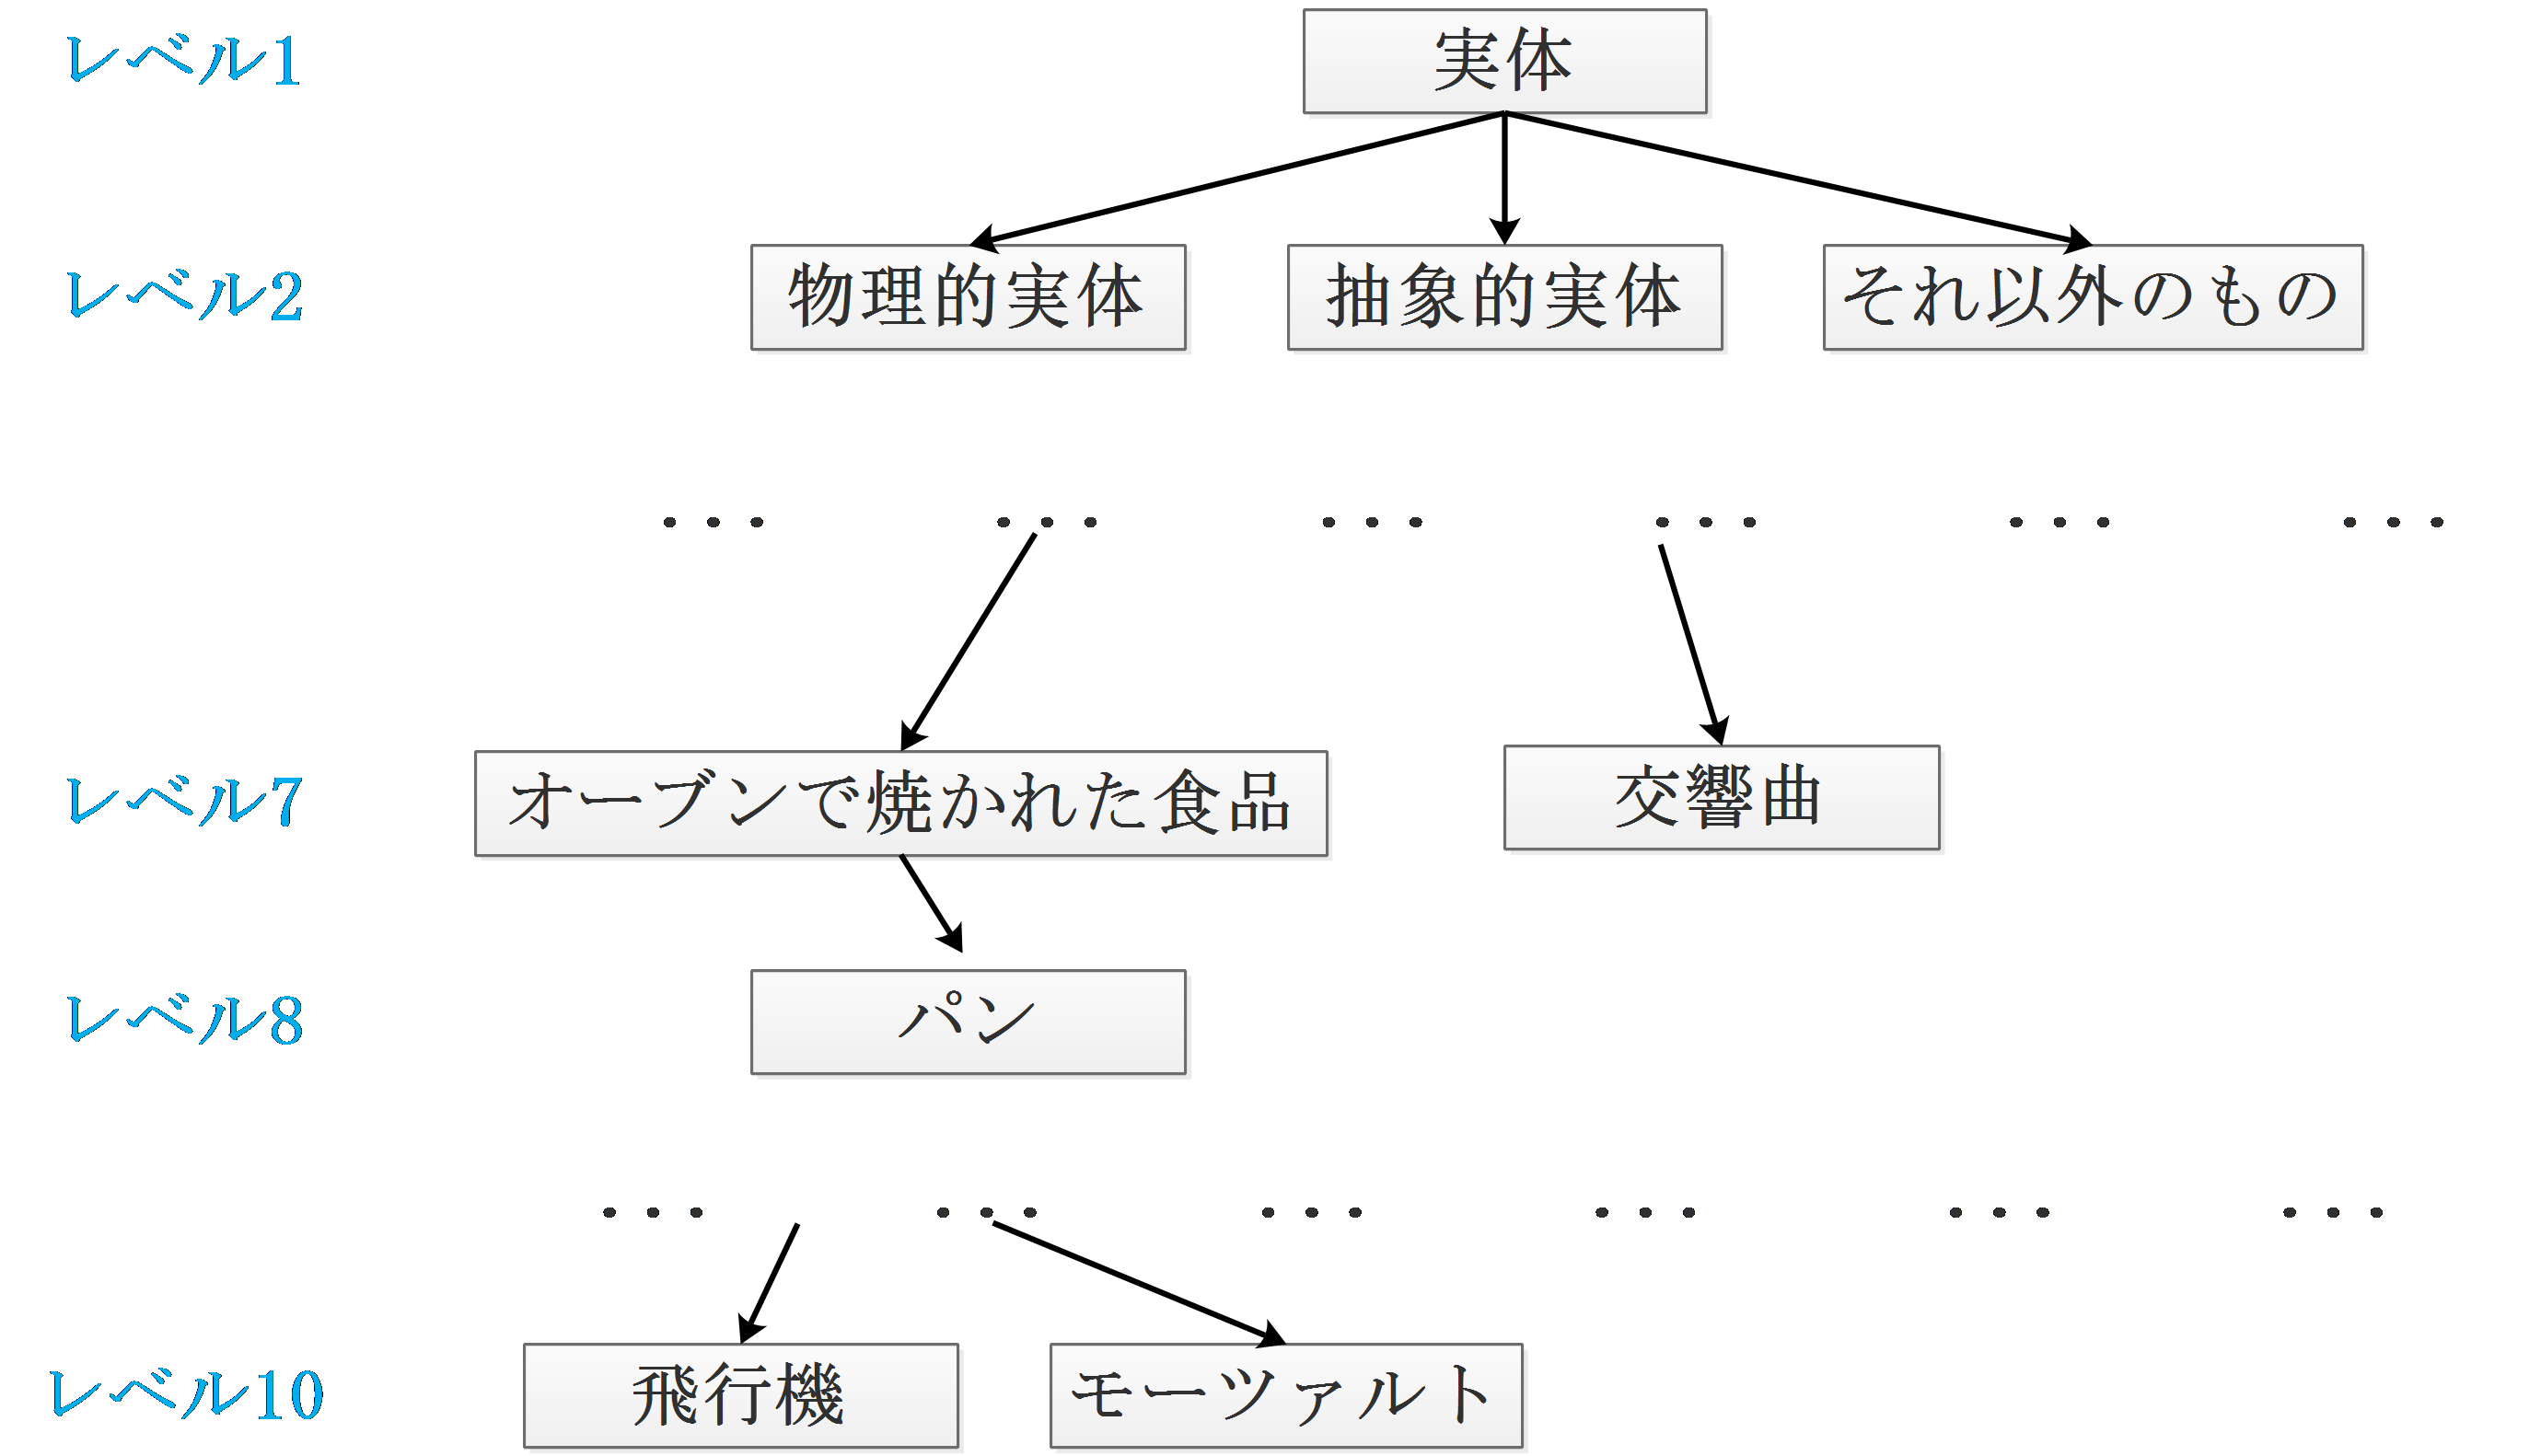
\includegraphics[width=\columnwidth]{rk15.png}
		\end{column}
	\end{columns}
\end{frame}

\begin{frame}{Embellishing Text Search Queries to Protect User Privacy \cite{embellishing2010}}
	\begin{block}{単語間距離関数:$dist_{WordNet}$}
		単語$a$の$synset$を$A$とし単語$b$の$synset$を$B$とする.
		$synset \, A$と$synset \, B$間の最短パスを$PATH(A,B)$とする.
		WordNetによる単語間距離関数$dist_{WordNet}$とは
		\begin{equation}
			dist_{WordNet}(a,b) = |PATH(A,B)|
		\end{equation}
	\end{block}
\end{frame}

\begin{frame}{Embellishing Text Search Queries to Protect User Privacy \cite{embellishing2010}}
	\begin{block}{問題点}
		\begin{itemize}
			\item 	WordNetに含まれていない専門用語が多い
			\item 	単語バケットを作るときは単語間で距離しか配慮していない.
		\end{itemize}
	\end{block}
\end{frame}

\begin{frame}{On masking topical intent in keyword search \cite{masking2014}}
	\begin{block}{}
		\begin{itemize}
			\item 	Hash関数を用いてダミー質問が属するトピックを決定する
			\item	LDAを用いてトピック$t$に単語$w$の出現確率$Pr(w|t)$を計算し、$Pr(w|t)$からランダムで取り出した単語の集合をダミー質問にする
		\end{itemize}
	\end{block}
\end{frame}

\begin{frame}{latent Dirichlet allocation  \cite{latent2003}}
	\begin{block}{}
	\end{block}
\end{frame}

\begin{frame}{On masking topical intent in keyword search \cite{masking2014}}
	\begin{block}{問題点}
		\begin{itemize}
			\item 	単語数が多いデーターベースのLDA計算
			\item	真の質問が同じトピックに属するとき対応するダミー質問も同じトピックに属するが,これだけで安全だと言えるか
		\end{itemize}
	\end{block}
\end{frame}

\begin{frame}{SimAttack \cite{simattack2016}}
\fontsize{12pt}{7.2}\selectfont
	\begin{block}{類似度:$sim$}
	\begin{algorithmic}[1]
		\REQUIRE 質問$q$,ユーザープロフィール$P_u$,スムージングパラメータ:$\alpha$
		\FOR {$q_i \in P_u$}
		\STATE $coef[i] \leftarrow 2 \cdot |q \cap q_i| \cdot \frac{1}{|q|+|q_i|}$
		\ENDFOR
		\STATE $coef \gets sort(coef)$
		\STATE $sim \gets coef[0]$
		\FOR {$i \in [1,|P_u|]$}
		\STATE $sim \gets \alpha \cdot coef[i] + (1 - \alpha) \cdot sim$
		\ENDFOR
		\ENSURE $sim$
	\end{algorithmic}
	\end{block}
	\begin{block}{$SimAttack$}
	\begin{algorithmic}[1]
		\REQUIRE 質問集合$Q$,ユーザープロフィール$Pu$,スムージングパラメータ:$\alpha$
		\STATE $q^* = \argmax_{q \in Q}sim_{q,Pu}$
		\ENSURE $q^*$
	\end{algorithmic}
	\end{block}
\end{frame}

\begin{frame}{既存研究}
    \begin{block}{}
        \fontsize{11pt}{7.2}\selectfont
		\center
        \begin{tabular}{cccc}
        \noalign{\hrule height 1pt}
         & 潜在意味分析手法 & 質問列の対応 & 長い質問の対応  \\
        \hline
        \cite{providing2009} & LSI   & X & X \\ 
		&&&\\
        \cite{embellishing2010} & WordNet  & X & O \\
		&&&\\
        \cite{masking2014} & LDA & O & O \\
        \noalign{\hrule height 1pt}
        \end{tabular}
    \end{block}
\end{frame}

\section{提案手法}
\begin{frame}{単語ベクトル}
    \begin{block}{単語ベクトル$l_t$}
		$T$を全てのトピックの集合とし$W$を全て単語の集合とする.
		トピック$t$の単語ベクトル$l_t$とは
		\begin{equation}
		\begin{aligned}
			& l_t  = \{w_1,w_2, \dots , w_{|W|}\}, \\
			& \forall w \in l_t, w \in W \\
			& \forall  1 \leq i \neq j \leq, w_i \neq w_j \\
			& \forall 1 \leq i < j \leq |W|,rscore(w_i,t) \geq rscore(w_j,t) 
		\end{aligned}
		\end{equation}
    \end{block}
\end{frame}

\begin{frame}{トピック間の距離}
    \begin{block}{トピック間の$cos$距離関数$dist_{cos}$}
		$l_{t_1},l_{t_2}$をトピック$t_1,t_2$の単語ベクトルとする.
		トピック$t_1,t_2$の$cos$距離関数$dist_{cos}$とは
        \begin{equation}
			dist_{cos}(t_1,t_2) = dist_{LSA}(l_{t_1}[1:1000],l_{t_2}[1:1000])
        \end{equation}
    \end{block}
    \begin{block}{トピック間の$coef$距離関数$dist_{coef}$}
		$l_{t_1},l_{t_2}$をトピック$t_1,t_2$の単語ベクトルとする.
		トピック$t_1,t_2$の$coef$距離関数$dist_{coef}$とは
        \begin{equation}
			dist_{coef}(t_1,t_2) = 1 - \frac{l_{t_1}[1:1000] \cap l_{t_2}[1:1000])}{1000}
        \end{equation}
    \end{block}
\end{frame}

\begin{frame}{流れ}
	\fontsize{10pt}{7.2}\selectfont
	\center
	\begin{tabular}{ccccc}
	\noalign{\hrule height 1pt}
	 && 文章単語行列 &&  \\
	\hline
	&tfidf & LSI   & LDA& \\ 
	\hline
	 && トピック単語ベクトル(辞書) && \\  
	\hline
	 cos-近い& cos-遠い & データベース分割 & coef-近い & coef-遠い \\
	\hline
	&&トピック分類&& \\
	\hline
	&同じ位置&同じ位置+ノイズ&zipf分布& \\
	\hline
	&&ダミー質問&& \\
	\noalign{\hrule height 1pt}
	\end{tabular}
\end{frame}

\section{プライバシー分析}
\begin{frame}{SimAttack New}
\fontsize{12pt}{7.2}\selectfont
	\begin{block}{$SimAttack_{New}$}
	\begin{algorithmic}[1]
		\REQUIRE 質問集合列$\hat{Q}=\{ Q_1,Q_2, \dots , Q_n\}$,スムージングパラメータ:$\alpha$
		\FOR {$j \in |Q_1|$}
			\STATE $\hat{Pu}[j] = Q_1[j]$
			\STATE $\hat{Put}[j] = \Phi$
			\STATE $d[j] = 0$
		\ENDFOR
		\FOR {$i \in [2,n]$}
			\FOR {$j \in |Q_i|$}
				\STATE $\hat{Put}[j] = \argmax_{Pu \in \hat{Put}}sim_{Q_i[j],\hat{Put}[j]}$
			\ENDFOR
			\STATE $q^*_i = \argmin_{Q_i[j] \in Q_i}sim_{Q_i[j],\hat{Put}[j]}$
			\FOR {$j \in |Q_i|$}
				\STATE $\hat{Pu}[j] = \hat{Put}[j] \cap Q_i[j]$
			\ENDFOR
		\ENDFOR
		\ENSURE $q^*$
	\end{algorithmic}
	\end{block}
\end{frame}

\begin{frame}{メイントピック攻撃}
	\begin{block}{$Main Topic Attack$}
	\begin{algorithmic}[1]
		\REQUIRE 質問集合$Q$
		\IF {$Q = \{q_1,q_2 , \dots , q_{|Q|} \} $}
			\STATE $q^* = \argmax_q \max_t rscore_{LSA}(q,t)$
		\ELSIF {$Q = \{w_1^1,w_1^2, \dots , w_1^k , \dots , w_n^k\}$}
			\STATE $t^* = \argmax_t rscore_{LSA}(Q,t)$
			\FOR {$i \in \{1,2, \dots , n\}$}
				\STATE $w_i^* = \argmax_{w_i^j} rscore_{LSA}(w_i^j,t^*)$
			\ENDFOR
			\STATE $q^* = \{ w_1^*,w_2^*, \dots , w_n^*\}$
		\ENDIF
		\ENSURE $q^*$
	\end{algorithmic}
	\end{block}
\end{frame}

\begin{frame}{実験}
	\begin{center}
		\begin{tabular}{|c|c|}
		\noalign{\hrule height 1pt}
		重複を除いた単語数 & $2,973,096$  \\
		文章数 & $3,496,253$ \\
		質問数 & $2,908$ \\
		質問平均単語数 & $21.0$ \\
		国際特許分類数 & 623 \\
		\noalign{\hrule height 1pt}
		\end{tabular}
	\end{center}
\end{frame}

\begin{frame}{実験}
\fontsize{11pt}{7.2}\selectfont
	\begin{block}{LSA ランダムトピック}
	\center
		\begin{tabular}{|c|c|c|c|c|c|}
		\noalign{\hrule height 1pt}
		評価方法:ダミー質問数  & 3 & 4 & 5 & 6 & 7i    \\
		SimAtt New &  & 78.2 & 78.5 & 77.3 & 63.8 \\
		SimAtt LSA & 65.5 &55.6 & 50.8 & 48.2 & 50.7 \\
		Maintopic & 75.2 & 72.3 & 67.6 & 64.2 & 58.5 \\ 
		100番までの検索結果重複率 & 6.0 & 1.9 & 2.0 & 1.9 & 1.9 \\
		\noalign{\hrule height 1pt}
		\end{tabular}
	\end{block}
	\begin{block}{同トピック}
	\center
		\begin{tabular}{|c|c|c|c|c|}
		\noalign{\hrule height 1pt}
		評価方法  & SimAtt New & SimAtt LSA  & Maintopic & 重複率  \\
		tfidf  & 25.1 & 25.0 & 25.1 & 28.5 \\
		LSA  & 27.6 & 27.0 & 25.8 & 20.7 \\
		LDA  & 25.8 & 24.6 & 24.8 & 32.3 \\
		\noalign{\hrule height 1pt}
		\end{tabular}
	\end{block}
    \begin{block}{データベース分割(8)}
    \center
        \begin{tabular}{|c|c|c|c|c|}
        \noalign{\hrule height 1pt}
		評価方法  & SimAtt New & SimAtt LSA  & Maintopic & 重複率  \\
        データベース分割(8)  & 52.3 & 11.6 & 42.1 & 1.5 \\
        \noalign{\hrule height 1pt}
        \end{tabular}
    \end{block}
\end{frame}

\begin{frame}{実験}
\fontsize{11pt}{7.2}\selectfont
    \begin{block}{LSAトピック分類方法}
    \center
		\begin{tabular}{|c|c|c|c|}
        \noalign{\hrule height 1pt}
        評価方法  & SimAtt LSA  & Maintopic & 重複率  \\
        coef-far  & 88.7 & 69.2 & 5.2 \\
        coef-near & 35.5 & 28.2 & 8.5 \\
        \noalign{\hrule height 1pt}
        \end{tabular}
    \end{block}
\end{frame}


\section{まとめ}
\begin{frame}{まとめ}
	\begin{block}{}
	\end{block}
\end{frame}

\section{参考文献}
\begin{frame}[t,allowframebreaks]{Bibliography}
\fontsize{8pt}{7.2}\selectfont
\bibliographystyle{alpha}
\bibliography{thesis}
\end{frame}

\end{document}

